\chapter{Realisierung}
In diesem Kapitel wird näher auf das Zusammenspiel von Sensorik (Kinect) und Aktorik (Nao) eingegangen. Zunächst wird die Idee der Softwarearchitektur vorgestellt. Im Anschluss daran, wird auf die entworfenen Algorithmen näher eingegangen.

\todo{Wahl Programmiersprache (warum? ->Kinect und Nao gleich, Visual Studio)}
\todo(Wahl Bibliothek, warum?...)
\todo{Erklärung Webots, Choreograph, Nao Verbindung, Libraries...}
\todo{Danach -> echter Nao im Laber -> Unterschied zur Simulation}
\todo{Laborbedingungen Steuerungen, Vor- und Nachteile der Bedienung}

%%
%
%	Erklärung der einzelnen Module + was ist der Knackpunkt?
%		MainWindow -> starten & initialisieren
%			!Annotation! := Erläutern Thread Konzept C# .xaml + .xaml.cs
%							bzw. Dispatcher (security != Java)
%		Interfaces 		-> 	austauschbar & fokus auf relevante Daten => Winkel
%							Wiederverwendbar für Nao UND gui
%		KinectHandler	-> 	Input der Anwendung
%		Calculation 	-> 	Threading, Berechnungen CPU-Intensiv
%						-> 	Errechnet aus Skelett Winkel
%						-> 	Versorgt GUI, Nao mit Winkelwerten
%						-> 	Werte vorfiltern (Filter erklären)
%		NaoHandler 		-> 	Output der Anwendung
%							Mapping Kinect-Nao-Raum, Ruckeln vermeiden
%
%	Workflow darstellen (evtl. Flussdiagram + Erläuterung)
%		Programm starten über MainWindow
%		Erzeugt Frame und startet/initialisiere alle Submodule
%			Init KinectHandler
%			Init NaoHandler
%			Init Berechnungen
%		Warte auf Skelett...
%		Skelett erkannt -> starte Berechnungen
%		Zeige Skelett im Hauptframe an
%		Für jedes aktualisierte Skelett
%			Errechne Winkel
%			Winkel filtern
%			Aktuellen Status aktualisieren -> Observer Pattern
%				GUI
%				NaoHandler
%		
%%
\section{Architektur}\label{k:Architektur}
Die Architektur der Anwendung kann grob in zwei Teilbereiche gegliedert werden, den Sensorik- und den Aktorik-Bereich.
Der Sensorteil ist dafür zuständig, die entsprechenden Gesten des Benutzers zu ermitteln und zu verarbeiten. Der Aktorteil der Anwendung ist dafür zuständig die Werte entsprechend auf die Wertebereiche des Nao-Koordinatensystems zu transformieren und diese dem Roboter zu übermitteln.


\subsection{Interfaces}
Als Schnittstelle zwischen der Erkennung und der Ausführung der Armpositionen wird essenziell die Methode \textit{updateAngles} vom Interface \textit{ISkeletonAngles} verwendet. Diese stellt alle benötigten Winkel wie Shoulder Pitch, Shoulder Roll, Ellbow Roll, Elbow Yaw bereit. Somit kann dieses Interface von allen Klassen implementiert werden, die immer die aktuellen Werte benötigen, wie der NaoHandler und die GUI.

\subsection{Klassendiagramm}

\subsection{Flussdiagramm: Winkelerkennung}

\todo{Architekturidee: Input, Verarbeitung(evtl. Filter->Probleme Ruckeln?), Output, }
\section{Prototypen}
Im Rahmen der Entwicklung des finalen Endprogramms wurden mehrere Prototypen entwickelt, um sich erstens in die einzelnen SDK einzuarbeiten und zweitens die Prototypen zu erweitern und zu vereinen. Diese Prototypen werden hier vorgestellt.

\subsection{Erster Kinect-Prototyp}
Anhand der obigen Überlegungen wurde der erdachte Algorithmus zunächst via eines Prototyps implementiert. Dieser sollte an erster Stelle dazu dienen, das Microsoft Kinect SDK näher kennenzulernen. Der erste Prototyp erfüllte folgende Funktionen:
\begin{itemize}
	\item Connect-Disconnect von Kinect
	\item Winkelerkennung des Benutzers mit Anzeige in Grad
	\item Anzeige des Kamerabildes mit Gelenkkennzeichnung von Kopf und Armen
\end{itemize}

\subsection{Erster Nao-Prototyp}
Zur Einarbeitung in das Nao-SDK wurde eine Anwendung erstellt, die verschiedene Armwinkel an den Roboter übermitteln können.

In Bild \myref{f:nao_prototyp1} sind verschiedene Eingabefelder zu sehen. In die oberste wird die IP-Adresse eingetragen, die dem zu benutzenden Nao (hier: lokal in Webots) entspricht. Bei einem Klick auf den Button \textit{Connect} wird im Hintergrund ein neuer Proxy geöffnet. Wenn die Verbindung erfolgreich aufgebaut wurde, wird auch der Button \textit{Move} klickbar.
\begin{figure}[H]						
	\centering							
	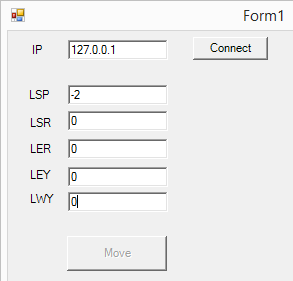
\includegraphics[scale=0.8]{Bilder/nao_prototyp1.PNG}
	\caption{Erster Nao-Prototyp}						
	\label{f:nao_prototyp1}						
\end{figure}
\noindent
In die anderen Felder müssen die einzelnen Winkel (im Bogenmaß) für die Gelenke (LSP = LeftShoulderPitch, LSR = LeftShoulderRoll, usw.) eingetragen werden. Bei Klick auf den Button \textit{Move} werden die einzelnen Winkel des linken Arms in die Position der eingetragenen Werte gefahren. In diesem Fall hebt der Roboter den linken Arm nach oben an, da \textit{LSP} mit -2rad definiert ist und dies im Nao-Gelenkraum einem Winkel von $-115^{\circ}$ entspricht (Siehe Kapitel \ref{tab:Lgelenkraum} und Abbildung \ref{f:gelenkraumL}). Ist ein angegebener Winkel nicht im Gelenkbereich wird die komplette Bewegung nicht ausgeführt (gilt nur für diesen Prototyp).

\subsection{Zweiter Prototyp}
Anhand der ersten Prototypen wurde das nun erworbene Wissen in eine gemeinsame Architektur eingebettet (Siehe \myref{k:Architektur}). Als Verbesserungen wurden alle benötigten Winkel auf zwei separaten Fenstern angezeigt, eines für jeden Arm. Auf der Fensteroberfläche wird nun das komplette Skelett über das RGB-Bild gelegt (siehe Abbildung \ref{f:programm}).


\subsection{Endprogramm}
Um den effektiven Algorithmus der Winkelerkennung noch effizienter zu gestalten, wurde noch ein Medianfilter implementiert, um die Ausreißer in den erkannten Winkeln zu eliminieren und somit die Messungenauigkeit der Gelenkpositionen zu verringern.
\newline
An der Oberfläche aus dem zweiten Prototyp wurde nicht mehr viel verändert. Lediglich eine Eingabemaske für die IP-Adresse des Nao-Roboters wurde hinzugefügt. Diese wird direkt bei Start des Programmes angezeigt.

\begin{figure}[H]						
	\centering							
	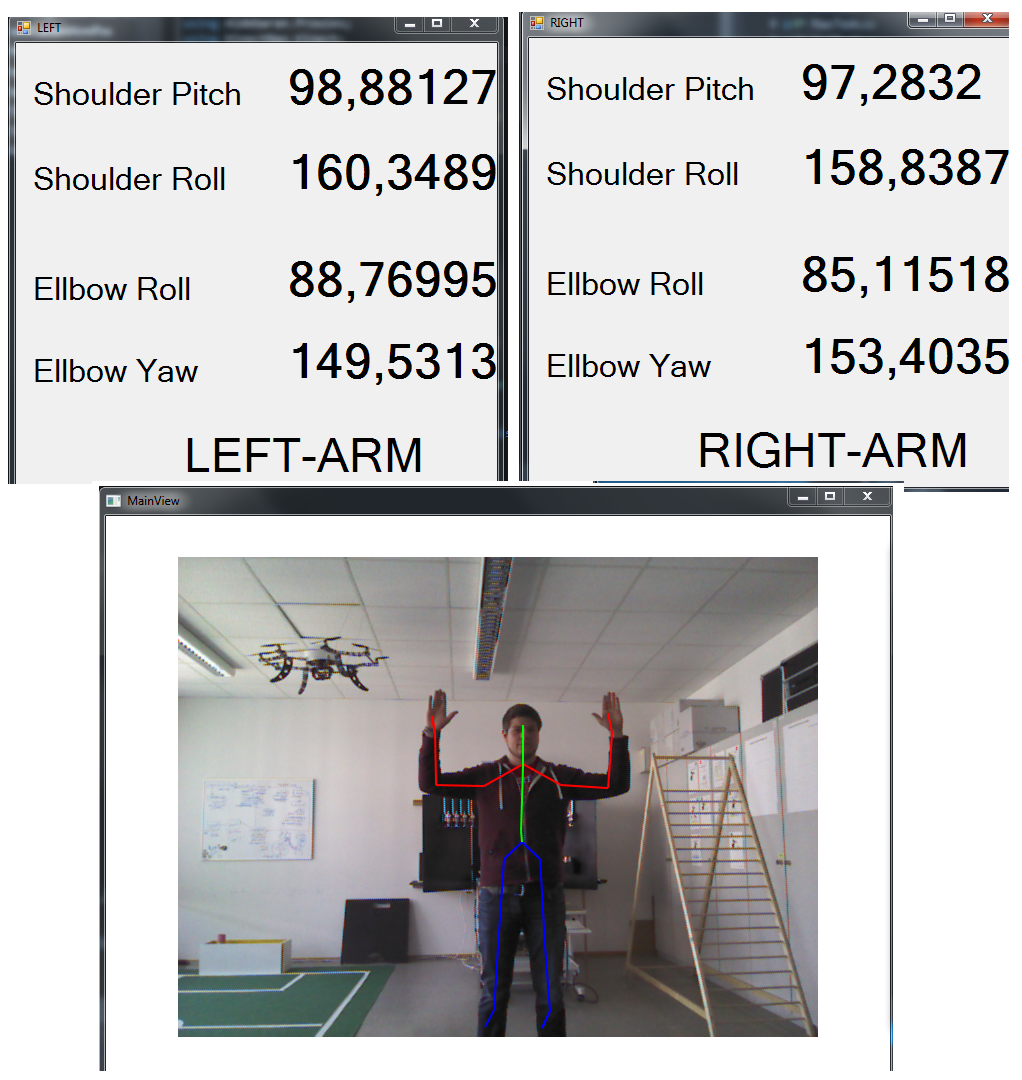
\includegraphics[scale=0.4]{Bilder/Programm.png}
	\caption{Fertige Applikation}						
	\label{f:programm}						
\end{figure}


%\todo{Screenshot von Prototypprogramm}